\section{固定候选池与失败路径分析}
\label{sec:frozen-pool}
为分离 H 位置与采样分布变化，历史机制实验在 MatMul128 和固定 target 下采集两个独立提案池，其三条比较路径使用同一历史 DLL；该计时不与本批主实验合并。初始化先通过真实 replay 得到完整决策，在后处理前冻结 trace；随后从基线完整后处理通过的固定父代生成单次变异子代。两个池分别有 64 条完整 trace（63 条唯一，7 个初始合法父代），以及 256 次提案中的 255 条完整 trace（238 条唯一，13 个初始合法父代）；后者另有一次未产生子代，保留记账，不补采样。这不是线上完整 GA 轨迹。

比较关闭 H、回放后 IR H、回放前 trace H 三条路径。第三条路径对所有未拒绝者继续 replay 和 IR H。CS 关闭以保持原始决策，每臂使用新的 Schedule、同一 replay seed 和 target 派生的完整七项 postproc 链。对象恢复重新绑定注册指令，不预先执行 replay。所有候选均有完整基线 oracle，包括 H 提前拒绝者；每个通过者的最终 IR 与采集 oracle 做结构相等检查。热身后轮换三臂顺序计时三轮，重复属于技术重复，不是三个独立搜索 seed。

\begin{table*}[tb]
\centering
\caption{固定完整 trace 池的 CPU 机制 pilot。拒绝/通过为每轮次数，时间为三轮候选路径总时间的中位数；不含采集与启动，不是 GPU 调优墙钟。}
\label{tab:frozen-pool}
\begin{tabular}{llrrrr}
\toprule
完整 trace & 路径 & H 拒绝 & Verify 拒绝 & 通过 & 时间 (s) \\
\midrule
64 & 无 H & 0 & 31 & 33 & 2.620 \\
64 & 回放后 H & 28 & 3 & 33 & 2.700 \\
64 & 回放前 H & 28 & 3 & 33 & 2.516 \\
\midrule
255 & 无 H & 0 & 128 & 127 & 16.328 \\
255 & 回放后 H & 111 & 17 & 127 & 16.152 \\
255 & 回放前 H & 111 & 17 & 127 & 15.758 \\
\bottomrule
\end{tabular}
\end{table*}

两个池均未观察到 H 误拒或 oracle 判定不一致。255 条池的 127 次通过对应 110 条唯一通过 trace；该经验安全证据不等于全空间证明或 GPU 数值正确性认证。该池初始化的 128 条完整 trace 中 H 拒绝 103 条，变异的 127 条中仅拒绝 8 条，不应把总体拦截量归为 GA 收益。64 条池还在独立进程中从原文件复评三轮，通过集合、拒绝位置与最终 IR 仍一致；这验证冻结池可复评，不增加独立采样数。

\begin{figure*}[tb]
\centering
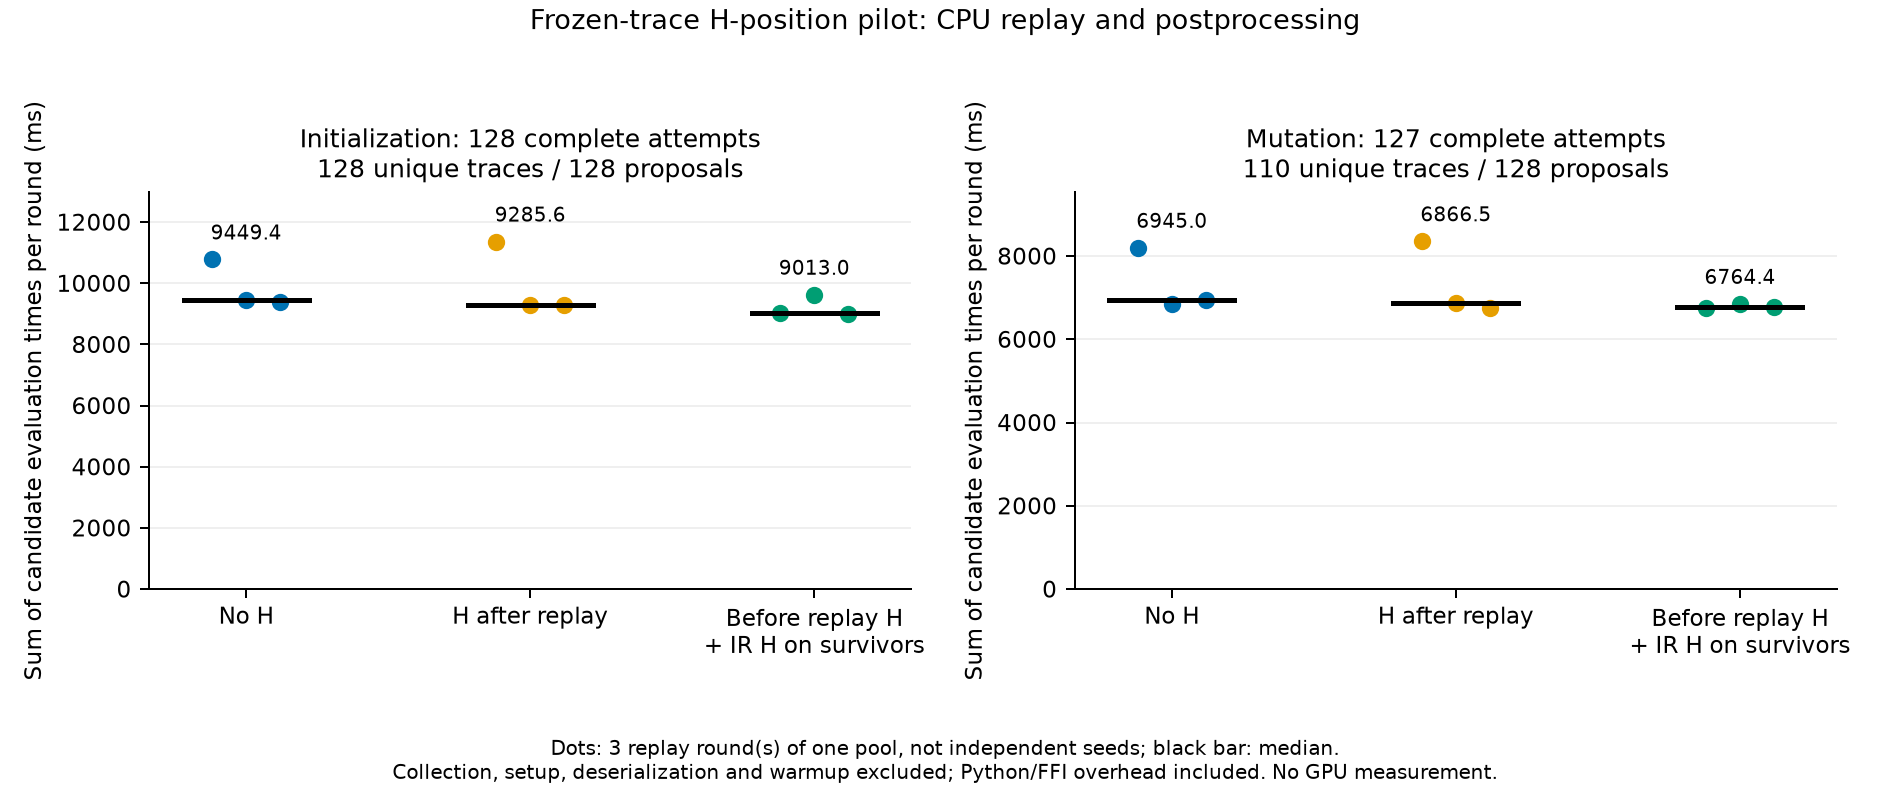
\includegraphics[width=\linewidth]{figures/p1_fixed_pool/pilot02/fixed_pool_round_timing.png}
\caption{255 条完整 trace 池的分阶段 CPU 路径时间。散点为同池三次计时，黑线为中位数；包含 H 检查、replay、postproc 与编排成本，排除采集、对象恢复、热身及结构相等核验。变异阶段的 128 次提案仅产生 127 条完整 trace。}
\label{fig:frozen-pool}
\end{figure*}

回放前 H 的总时间中位数相对无 H 约减少 $4.0\%/3.5\%$，但不能据此宣称稳定端到端收益。尤其在较大池中，111 条早拒者占完整候选的 $43.5\%$，其基线完整处理时间却仅为每轮 $0.609$--$0.691$ s，占基线总时间 $3.64\%$--$3.80\%$；这些候选的 Verify 合计只有 $3.55$--$4.67$ ms。其余 144 条幸存者的 Verify 合计为 $14.86$--$17.36$ s。源码中 Verify 先检查线程契约、失败直接返回，再对剩余候选 lowering，与该现象一致。因此少掉 111 次 Verify 不等于省掉 111 次完整 lowering。

进一步按同一候选 ID 分区可见，H 放行但最终 Verify 失败的 17 条仅占候选的 $6.7\%$，却占基线总路径的 $85.54\%$--$86.14\%$；127 条通过者占 $10.22\%$--$10.66\%$（图~\ref{fig:cost-cohorts}）。其中 8 条失败的 Verify 单条中位耗时为 $1.689$--$1.817$ s，贡献基线总路径的 $84.76\%$--$85.39\%$。这是原始三个技术重复上的成本集中现象，不是已经实现的加速比，也不是针对全部工作负载的总体估计。

\begin{figure*}[tb]
\centering
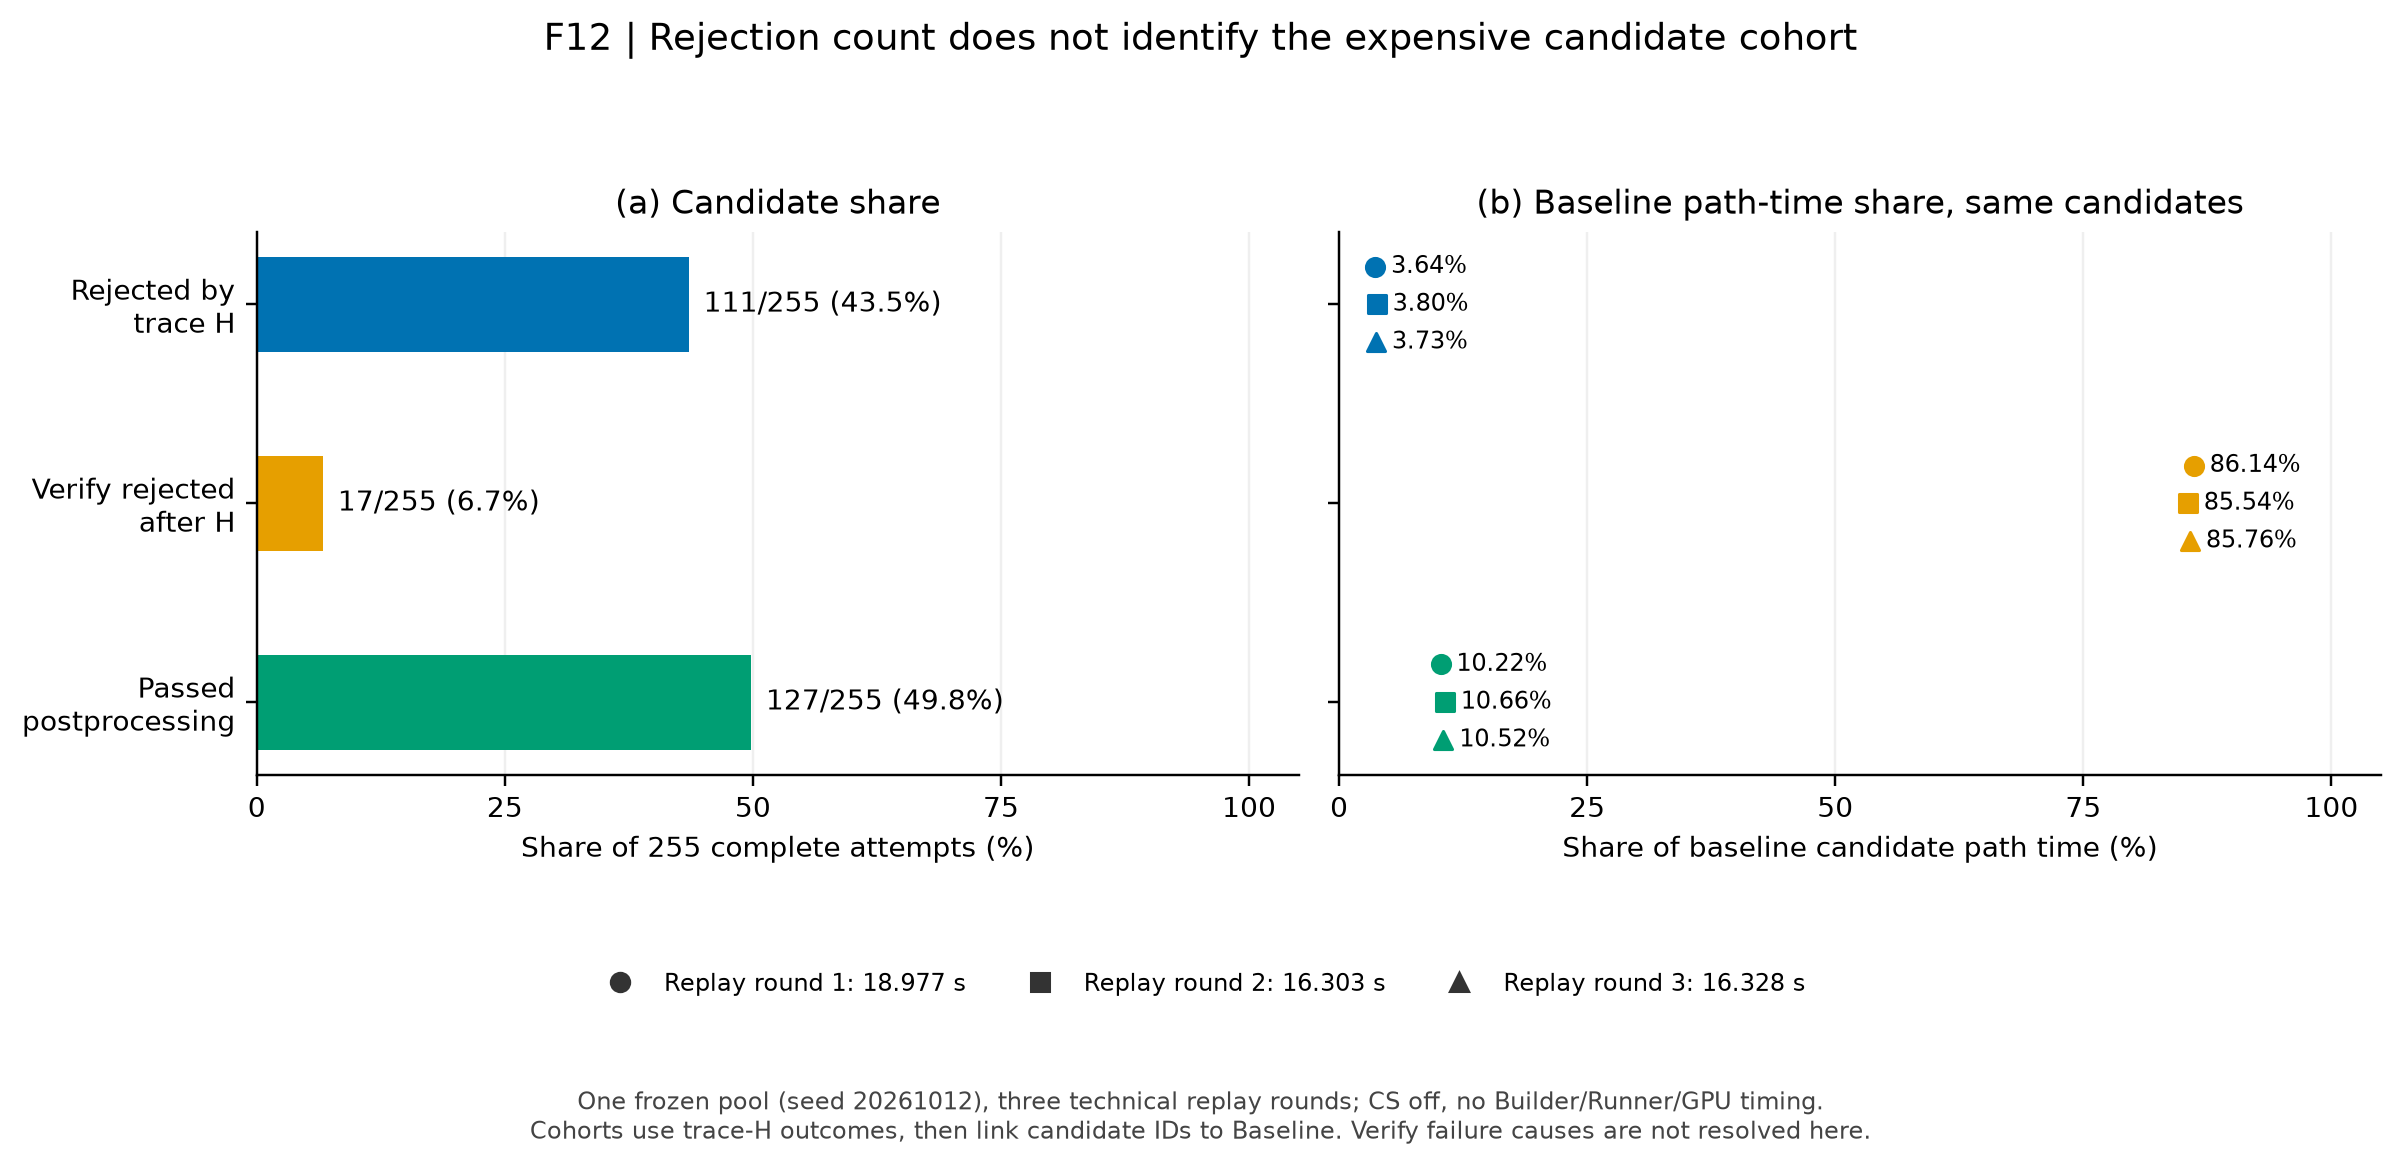
\includegraphics[width=\linewidth]{figures/pilot_mechanism_20261008/f12_fixed_pool_cost_cohorts.png}
\caption{同一固定池的候选数量与基线处理成本。左为按 H 路径确定的三组候选比例，右为回查基线同候选的各轮路径时间占比。17 条残余失败贡献主要成本；三个点为同池技术重复，不是独立搜索 seed，且不含 GPU 测量。}
\label{fig:cost-cohorts}
\end{figure*}

为定位失败，我们仅增加读取 Verify 首个失败类别的只读接口，并编译独立诊断 DLL（SHA256 前缀 \texttt{c2853006ea72}）。在原 255 条完整 trace 上重新执行三条路径，共 765 次判定均与旧 oracle 一致，381 次通过结果的最终 IR 均结构相等。新诊断分类为 111 次线程契约失败、9 次共享内存失败、8 次 lowering 异常及 127 次通过；H 恰好提前拒绝上述 111 次线程失败。随后只对 17 条残余失败进行独立 pass 观察，保持原 PassContext 参数与 lowering 顺序：8 条长尾的最深未闭合 pass 均为 \texttt{s\_tir.InjectSoftwarePipeline}，9 条共享内存失败则完成 lowering 后在资源检查中被拒。诊断计时包含接口与观察器开销，未替换原固定池性能数据；接口只报告首个失败原因，不等于列出了全部违规。

对观察器保存的精确 pass 输入进一步单独调用原软件流水线变换，8 条均重现同一结构错误：流水线阶段注释含 3 项，而实际主体含 4 个块。输入中两个共享内存加载后分别出现归约初始化与更新块，原 3 项注释不再匹配该结构。该证据说明主要长尾的直接触发点是变换契约不一致；它并不排除修复结构后仍存在资源超限。

为区分结构错误与后继资源失败，我们在原 255 条 trace 上观察归约分解前后的 IR，再对上述 8 条分别执行三种反事实：只删除流水线的阶段、顺序和异步阶段注释；将本模板的外层归约因子由 1 改为 2，并将一个可整除的内层因子减半以保持乘积；在原归约后处理之前显式将零初始化提到带注释的单位循环外。原始对照的 255 次状态与首个失败原因均不变，127 次通过结果与原 oracle 的 IR 结构相等。8 条原候选均在 \texttt{RewriteReductionBlock} 前含 3 个直接主体项，之后变为 4 项，而注释保持 3 项；改分块和外提初始化两种干预使所观察主体保持 3 项。这里的直接主体计数仅用于本批归因，不是镜像所有 lowering 变换的通用剪枝判据。

\begin{table*}[tb]
\centering
\caption{同一批 8 条 lowering 失败候选的反事实。三种修改均消除了流水线异常，但不一定消除后继共享内存超限；数量不是独立搜索 seed。}
\label{tab:pipeline-counterfactual}
\begin{tabular}{lrrr}
\toprule
干预 & lowering 异常 & shared 超限 & 完整后处理通过 \\
\midrule
原始候选 & 8 & 0 & 0 \\
关闭流水线注释 & 0 & 7 & 1 \\
外层因子 $1\to2$，乘积不变 & 0 & 8 & 0 \\
零初始化外提 & 0 & 8 & 0 \\
\bottomrule
\end{tabular}
\end{table*}

表~\ref{tab:pipeline-counterfactual} 中唯一通过者为关闭流水线后的 \texttt{mutation-0037}。该程序在同一 RTX 3050 Ti Laptop GPU 上经真实 CUDA 编译，使用三组正态随机输入、一组均匀随机输入、单位矩阵与零矩阵两类结构化输入，并分别以 NaN 和常数初始化输出，共 12 次数值检查均通过。参考为独立 NumPy FP64 矩阵乘，绝对与相对容差均为 $2\times10^{-4}$；最大绝对误差为 $1.979\times10^{-5}$。这是单个修复程序的正确性证据，不是性能测量或通用修复证明。另有单位长度、短于流水线阶段数及动态短循环三项原生变换测试通过，因此不能按短循环长度直接扩展硬筛。

这些结果要求将“当前编译契约不兼容”与“硬件资源不可行”分开。早拒该结构可以避免已知异常路径，却不能被解释为排除了所有潜在好解；若引入修复，需同时提供使用相同修复的基线，才能将修复收益与 CS/H 收益分离。保持流水线的两种修复仍全部受到共享内存限制，后续应验证可靠资源界或限定结构的前置检查，而非仅以异常消失作为验收。

这一结果提示应按\emph{剩余无效工作的成本}而非单纯拒绝比例选择扩展约束。初始化完整决策已在采集时支付首次 replay，两个池的采集总成本分别为 3.621/21.958 s，启动成本为 90.644/84.497 s，均另列。故上述前移收益仅属于完整决策的复评路径，不能直接外推为线上初始化跳过首次 replay，也不构成新增 GPU 性能结果。

